
\documentclass[12pt]{article} 

\usepackage[utf8]{inputenc}
\usepackage[english]{babel}

\usepackage{graphicx}
\usepackage[labelformat=empty]{caption}

\usepackage{geometry} 
\geometry{a4paper}

\usepackage{fancyhdr} 
\pagestyle{fancy} 
\renewcommand{\headrulewidth}{0pt}
\lhead{}\chead{}\rhead{}
\lfoot{}\cfoot{\thepage}\rfoot{}

\usepackage{sectsty}
\allsectionsfont{\sffamily\mdseries\upshape}

%============================================================================================================
\begin{document}
\title{Operating Systems - Report on the Linux Systems}
\author{Samuel, Andersson, Johan Dahlberg, Eric Falheim, \\Camilla Heiding, Xuan Hoang, Amer Hodzic}
\date{Today}
\maketitle

\newpage
\tableofcontents
\newpage

\section{Linux History} %Written by
\subsection{The making of Linux}
git gud - Linus Torvalds.

\subsection{The kernel}
The kernel is the core of the operating system and make communication possible to the hardware.
It can exist many kernels in the same system. And in the case of a failure, when updating a kernel,
you can always boot the system with an older version that was working.

\begin{figure}[h]
  \begin{center}
    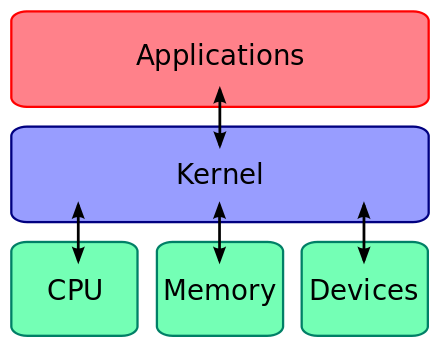
\includegraphics[scale=0.5]{imgs/structure}
    % https://blog.digilentinc.com/demystifiying-the-linux-kernel/
    \caption{Kernel interfacing hardware and user-space.}
  \end{center}
\end{figure}

\subsection{Linux licensing}
The Linux kernel is distributed under the GNU General Public License (GPL). 
This means that anyone can download the kernel for free to use however they choose.
If you modify the kernel and make a derivative of it, however, it must be distributed with the same licensing terms.
So whenever anyone modifies the code and adds their own standard programs and tools in a packaged form, it could be called a new operating system.
This is the reason for the extremely many different "flavors" of Linux.

\section{Kernel Modules} %Written by
%man-pages fork()
A kernel module is a driver that can be loaded into the kernel dynamically, at boot-time or run-time,
to make communication between a device and hardware possible (via the kernel).
This makes the kernel more lightweight due to the fact that unused modules can be unloaded from the kernel, which frees up RAM.
Whenever a new module is loaded, there is no need to rebuild the kernel or reboot the system.

All modules can be found in the /lib/modules/ folder.
Working with modules is easy in Linux. There are commands you can run from the CLI to load, unload and list modules.
\begin{itemize}
  \item lsmod - lists the loaded modules.
  \item modprobe \textbf{[-r]} \textit{module\_name} - will load or unload named module depending on the flag -r.
  \item insmod \textit{module\_name} - same as using modprobe without -r flag.
  \item rmmod \textit{module\_name} - same as using modprobe with -r flag.
\end{itemize}

\section{Process Management} %Written by
A process is a program in execution and it has it's own address space if it's spawned with the fork().
Processes can also be cloned with parameters, effectively telling the child whether it should share the parent's filesystem, memory space, signal handlers and open files.
Each process execute instructions sequentially, but can contain many threads. In Linux this is called a task. 
All threads share the same address space, and can therefore communicate via shared-memory.

\subsection{Process attributes}
A process is associated with a Process ID (PID) on creation, which will be unique for this process. 
Every process is spawned by a parent process (PPID) with a fork, and on creation the child-process memory space is identical to the parent's, but separate.
Who spawned the process and what group they belonged to is stored in Real User ID (RUID), Effective User ID (EUID), Real Group ID (RGID) and Effective Group ID (EGID).
The process has it's own priority which can be set from -20 (low) to 20 (high), by default it depends on recent CPU usage. 
In addition to this every process can be nice to other processes by hugging less resources. This value can be set between -20 to 19.
The TTY attribute tells us what terminal the process is connected to.

\subsection{Signals}
A signal in linux is like an interrupt, which happens due to an event. 
When a process recieves a signal, it will terminate if it isn't handling the signal.
\begin{itemize}
  \item SIGABORT - Process abort
  \item SIGALARM - Alarm clock
  \item SIGFPE - Floating point exception
  \item SIGHUP - Hangup
  \item SIGILL - Illegal instruction
  \item SIGINT - Terminal interrupt
  \item SIGKILL - Kill
  \item SIGPIPE - Write on a pipe with no reader
  \item SIGQUIT - Terminal quit
  \item SIGSEGV - Invalid memory segment access
  \item SIGTERM - Terminate
  \item SIGUSR1 and SIGUSR2 - User defined signals
\end{itemize}

\section{Scheduling} %Written by
%https://www.kernel.org/doc/html/latest/scheduler/index.html
\subsection{User-mode scheduling}
Completely fair scheduler (CFS).

\subsection{Kernel-mode scheduling}
First come first served  (FCFS) and Round Robin (RR).

%\section{Memory Management} %Written by
%https://www.kernel.org/doc/html/latest/admin-guide/mm/index.html

\section{File Systems} %Written by
\subsection{Files}
Everything is stored as files on Linux. Even directories, devices, sockets, pipes and symbolic links.
When showing information about a file you see something like "-rwx r-- r--". 
The first character determines the file's type. For regular files, a '-' is shown, and for directories a 'd' is shown. 
The remainder of the string determines the user-group-universal access-rights. 
For the example above, the user got read-write-execute rights, whereas the group and everyone else can just read that file.
This adds a level of protection to the system so only the processes and users with access-rights can read/modify/execute the file.

\subsection{inode}
An inode in UNIX-like systems are data-structures for files and directories. 
It could be simplified to a node in a tree. It would contain information about itself, it's parent-node and a list of child-nodes.

\subsection{Mounting}
There are no disk-drives in Linux, instead all devices are mounted on mounting points in the file-system. 
So installing a new hard-disk or inserting a USB-drive is treated the same way.
By mounting the device on an inode, you can treat the new device as a part of the whole file-system.

\subsection{File System Hierarchy Structure}
  The filesystem begins at the root /, where directories that divide the system logically is placed. Some examples:
  \begin{itemize}
    \item /bin - Contains binaries for the system. Easily accessed by the system via environment variable \$PATH.
    \item /boot - Files for booting the system, including the kernel.
    \item /dev - Contains the system's devices.
    \item /etc - Configuration files for the system.
    \item /lib - Modules, software libraries and information databases.
    \item /mnt - Mounting point for external devices.
    \item /net - Mounting point for remote file-systems.
    \item /home - Home directory containing every user's own home folder on the system. 
    \item /proc - Process file system
    \item /sbin - Binaries used by the administrator and the system.
    \item /usr -
    \item /tmp - A temporary directory that is emptied periodically, or when the system is shut down.
  \end{itemize}
 
\section{Input and Output} %Written by
\subsection{STDIN, STDOUT and STDERR}
\subsection{Redirection and Pipes}

\section{Interprocess Communication} %Written by
%https://opensource.com/article/19/4/interprocess-communication-linux-storage
\subsection{Shared memory}
\subsection{Pipes}
\subsection{Read-write to files}

%\section{Network Communications} %Written by

%\section{Security} %Written by

\section{Suggested topics to add}
\begin{itemize}
  \item file descriptors
  \item 
\end{itemize}

\end{document}

